\documentclass[12pt,a4paper,oneside]{report}
\usepackage[utf8]{inputenc}
\usepackage[english]{babel}
\usepackage{geometry}
\geometry{left=3cm,right=2cm,top=2.5cm,bottom=2.5cm}
\usepackage{amsmath}
\usepackage{amssymb}
\usepackage{booktabs}
\usepackage{graphicx}
\usepackage{tikz}
\usetikzlibrary{shapes.geometric, arrows.meta, positioning}
\usepackage{listings}
\usepackage{color}
\usepackage{setspace}
\usepackage{hyperref}
\hypersetup{
    colorlinks=true,
    linkcolor=blue,
    filecolor=magenta,      
    urlcolor=cyan,
    pdftitle={Master Thesis - Hybrid RAG},
}

% Definition of colors for code blocks
\definecolor{codegreen}{rgb}{0,0.6,0}
\definecolor{codegray}{rgb}{0.5,0.5,0.5}
\definecolor{codepurple}{rgb}{0.58,0,0.82}
\definecolor{backcolour}{rgb}{0.95,0.95,0.92}

\lstdefinestyle{mystyle}{
    backgroundcolor=\color{backcolour},   
    commentstyle=\color{codegreen},
    keywordstyle=\color{magenta},
    numberstyle=\tiny\color{codegray},
    stringstyle=\color{codepurple},
    basicstyle=\ttfamily\footnotesize,
    breakatwhitespace=false,         
    breaklines=true,                 
    captionpos=b,                    
    keepspaces=true,                 
    numbers=left,                    
    numbersep=5pt,                  
    showspaces=false,                
    showstringspaces=false,
    showtabs=false,                  
    tabsize=2
}
\lstset{style=mystyle}

\begin{document}

% ──────────────────────────────────────────────────────────────────────────────
% OUTER COVER PAGE
% ──────────────────────────────────────────────────────────────────────────────
\begin{titlepage}
    \begin{center}
        \large MINISTRY OF EDUCATION AND TRAINING \\
        \textbf{\large FPT UNIVERSITY} \\
        \vfill
        \vfill
        \begin{singlespace}
            \textbf{\Large RESEARCH AND DEVELOPMENT OF A CODEBASE QUERY SYSTEM BASED ON HYBRID-RAG ARCHITECTURE COMBINING KNOWLEDGE GRAPHS AND SEMANTIC SEARCH}
        \end{singlespace}
        \vfill
        \large by \\
        \large \textbf{Tran Tien Doat} \\
        \vfill
        \large A thesis submitted in conformity with the requirements \\
        for the degree of Master of Software Engineering \\
        \vfill
        \vfill
        \large \copyright\ Copyright by Tran Tien Doat 2026
    \end{center}
\end{titlepage}

% ──────────────────────────────────────────────────────────────────────────────
% INNER COVER PAGE
% ──────────────────────────────────────────────────────────────────────────────
\begin{titlepage}
    \begin{center}
        \large MINISTRY OF EDUCATION AND TRAINING \\
        \textbf{\large FPT UNIVERSITY} \\
        \vfill
        \vfill
        \begin{singlespace}
            \textbf{\Large RESEARCH AND DEVELOPMENT OF A CODEBASE QUERY SYSTEM BASED ON HYBRID-RAG ARCHITECTURE COMBINING KNOWLEDGE GRAPHS AND SEMANTIC SEARCH}
        \end{singlespace}
        \vfill
        \large by \\
        \large \textbf{Tran Tien Doat} \\
        \vfill
        \large A thesis submitted in conformity with the requirements \\
        for the degree of Master of Software Engineering \\
        \vfill
        \vfill
        \large Supervisor: \\
        \large \textbf{Assoc. Prof. Dr. Nguyen Van A} \\
        \vfill
        \large \copyright\ Copyright by Tran Tien Doat 2026
    \end{center}
\end{titlepage}

\pagenumbering{roman}

% ──────────────────────────────────────────────────────────────────────────────
% ACKNOWLEDGMENTS
% ──────────────────────────────────────────────────────────────────────────────
\chapter*{Acknowledgments}
\addcontentsline{toc}{chapter}{Acknowledgments}
I would like to express my deepest gratitude to my supervisor, Assoc. Prof. Dr. Nguyen Van A, for his invaluable guidance, continuous encouragement, and insightful feedback throughout the duration of this research. His dedication and expertise have been instrumental in the completion of this thesis.

I am also grateful to the faculty members of the Software Engineering Department at FPT University for their support and for providing a stimulating research environment. 

Finally, I would like to thank my family and friends for their unwavering support and encouragement during this academic journey.

\newpage

% ──────────────────────────────────────────────────────────────────────────────
% ABSTRACT
% ──────────────────────────────────────────────────────────────────────────────
\chapter*{Thesis Abstract}
\addcontentsline{toc}{chapter}{Thesis Abstract}
Querying codebases is a complex challenge because source code contains both syntactic structures (function call graphs, class inheritances, module definitions) and semantic meanings (documentation, implementation intent). Traditional Retrieval-Augmented Generation (RAG) applications that rely solely on vector similarity (Vector-only RAG) ignore the syntactic hierarchy of source code, leading to degraded performance when answering multi-hop or structural questions.

This thesis proposes **Hybrid-RAG**, a dual-retrieval architecture combining a Knowledge Graph (using FalkorDB) and a Vector Database (using Qdrant) to optimize codebase querying. The system integrates Tree-Sitter for Abstract Syntax Tree (AST) parsing and utilizes Reciprocal Rank Fusion (RRF) to merge structural and semantic candidate lists under a tight token budget. Experimental results evaluated on the LlamaIndex codebase show that Hybrid-RAG achieves a significant Hit Rate @5 increase from 0.308 (Vector-only) to \textbf{0.615} (+0.308) overall, and reaches \textbf{0.800} (+0.400) on deep 3-hop call graph queries. Furthermore, the system preserves local data sovereignty by running 100\% offline.

\newpage

\tableofcontents
\newpage

\listoftables
\addcontentsline{toc}{chapter}{List of Tables}
\newpage

\listoffigures
\addcontentsline{toc}{chapter}{List of Figures}
\newpage

% ──────────────────────────────────────────────────────────────────────────────
% LIST OF ABBREVIATIONS
% ──────────────────────────────────────────────────────────────────────────────
\chapter*{List of Abbreviations}
\addcontentsline{toc}{chapter}{List of Abbreviations}
\begin{singlespace}
\begin{tabular}{ll}
    \textbf{API} & Application Programming Interface \\
    \textbf{AST} & Abstract Syntax Tree \\
    \textbf{DB} & Database \\
    \textbf{ESB} & Enterprise Service Bus \\
    \textbf{FQN} & Fully Qualified Name \\
    \textbf{KG} & Knowledge Graph \\
    \textbf{LLM} & Large Language Model \\
    \textbf{MRR} & Mean Reciprocal Rank \\
    \textbf{MSE} & Master of Software Engineering \\
    \textbf{RAG} & Retrieval-Augmented Generation \\
    \textbf{RRF} & Reciprocal Rank Fusion \\
    \textbf{SOA} & Service-Oriented Architecture \\
    \textbf{SSE} & Server-Sent Events \\
    \textbf{VRAM} & Video Random Access Memory \\
\end{tabular}
\end{singlespace}
\newpage

\pagenumbering{arabic}

% ──────────────────────────────────────────────────────────────────────────────
% CHAPTER 1: INTRODUCTION
% ──────────────────────────────────────────────────────────────────────────────
\chapter{Introduction}

\section{Motivation}
In the modern software development lifecycle, software engineering professionals spend a significant portion of their work hours on program comprehension rather than writing new source code. Empirical studies indicate that developers spend approximately 70\% to 80\% of their daily effort reading, navigating, and understanding legacy codebases. The continuous growth of repository size, combined with high developer turnover and the prevalence of microservices, makes codebase onboarding and maintenance increasingly challenging. 

The advent of Large Language Models (LLMs) has opened new paradigms for software engineering assistants, offering capabilities like automated code generation, documentation, and answering natural language questions about code. However, applying state-of-the-art LLMs directly to large-scale enterprise repositories introduces major challenges:
\begin{enumerate}
    \item \textbf{Context Window Constraints and Cost:} Modern codebases often exceed millions of lines of code. Even with modern long-context LLMs, feeding an entire repository into the model's prompt is computationally infeasible, leads to high latency, and incurs prohibitive API costs.
    \item \textbf{The "Lost in the Middle" Phenomenon:} LLMs struggle to recall and synthesize information located in the middle of long prompts, leading to degraded reasoning quality.
    \item \textbf{Data Sovereignty and Privacy:} Enterprise source code represents critical intellectual property. Uploading proprietary codebases to third-party public cloud LLM providers poses severe privacy risks and compliance violations.
    \item \textbf{Structural and Syntactic Ignorance:} Code is not unstructured natural language; it is a highly structured, hierarchical graph of dependencies (class inheritances, function calls, module scoping). Traditional vector-based search engines slice source code into arbitrary text chunks, which breaks class boundaries and fails to capture structural relationships.
\end{enumerate}

To address these issues, this thesis presents a private, 100\% offline codebase query system based on a \textbf{Hybrid-RAG} architecture. It combines a Graph Knowledge Graph (using FalkorDB) with a Semantic Vector Database (using Qdrant) to perform relationship-aware codebase retrieval under a tight token budget, executed locally on Apple Silicon workstations using the Gemma 2 model.

\section{The Codebase Comprehension Problem in RAG}
Traditional Retrieval-Augmented Generation (RAG) models rely solely on vector similarity search (Vector-only RAG). In these systems, source code files are partitioned into text chunks based on character length or line count. Each chunk is embedded into a high-dimensional vector space using models like \texttt{nomic-embed-text}. When a user submits a query, the system retrieves the top-K chunks with the highest cosine similarity.

This approach fails on codebase understanding for two fundamental reasons:
\begin{itemize}
    \item \textbf{Chunk Fragmentation:} A simple character-based splitter can slice a function definition in half. The local context (such as import statements, class declarations, and variable definitions) is lost, which prevents the LLM from understanding the scope of the code block.
    \item \textbf{Relational Blindness:} Vector search cannot follow logical edges. If a developer asks: \textit{"Which classes inherit from \texttt{BaseRetriever} and what other methods do they call?"}, a vector database will only return snippets that contain the word "BaseRetriever". It cannot traverse the inheritance hierarchy or trace the call graph across different files.
\end{itemize}

Fusing a Knowledge Graph (KG) with vector retrieval (GraphRAG) bridges this gap. The graph stores the exact Abstract Syntax Tree (AST) structure of the codebase (e.g., \texttt{Class-[:INHERITS]->Class}, \texttt{Function-[:CALLS]->Function}), while the vector database stores the semantic meaning of the code blocks.

\section{Research Objectives}
The core objectives of this research are:
\begin{itemize}
    \item \textbf{Static Analysis via Tree-Sitter:} Design a reliable, incremental parser using Tree-Sitter to extract syntactic entities (Modules, Classes, Functions, Variables) and relationships (DEFINES, IMPORTS, CALLS, INHERITS) from Python codebases.
    \item \textbf{Global Entity Resolution:} Develop a resolver to clean import paths and resolve cross-file dependencies, establishing global relationships across different files.
    \item \textbf{AST-Aware Chunking:} Design a chunking strategy that partitions source code precisely along class and method boundaries, prepending structural scope headers to preserve context.
    \item \textbf{Parallel Retrieval and Fusion:} Build a dual-retrieval engine that queries the Knowledge Graph and Vector Database concurrently, fusing the outputs using the Reciprocal Rank Fusion (RRF) algorithm.
    \item \textbf{Context Assembly under Token Budgets:} Implement an assembler that prioritizes, deduplicates, and packs the most relevant code contexts into the LLM prompt.
    \item \textbf{Flexible Query Toggling:} Implement a user-controlled feature toggle (\texttt{codebase\_query}) in the REST API to allow users to switch between codebase-aware hybrid retrieval and raw LLM general chat.
    \item \textbf{Offline Execution:} Deploy the entire pipeline locally to ensure data privacy, using Gemma 2 and local database engines.
\end{itemize}

\section{Thesis Outline}
The remainder of this thesis is structured as follows:
\begin{itemize}
    \item \textbf{Chapter 2 (Literature Review \& Theoretical Foundations):} Reviews RAG architectures, property graphs, the RRF algorithm, and AST parsing concepts.
    \item \textbf{Chapter 3 (Proposed Hybrid-RAG System Architecture):} Details the design of the ingestion pipeline, AST-aware chunking, the FalkorDB graph schema, and the hybrid retrieval flow.
    \item \textbf{Chapter 4 (System Implementation):} Describes the technology stack, the REST API endpoints, the \texttt{codebase\_query} toggle, and OpenTelemetry observability.
    \item \textbf{Chapter 5 (Experimental Results \& Discussions):} Evaluates the system on the LlamaIndex codebase, comparing it to a Vector-only baseline.
    \item \textbf{Chapter 6 (Conclusions \& Future Work):} Summarizes the contributions and proposes future research directions.
\end{itemize}

\newpage

% ──────────────────────────────────────────────────────────────────────────────
% CHAPTER 2: LITERATURE REVIEW & THEORETICAL FOUNDATIONS
% ──────────────────────────────────────────────────────────────────────────────
\chapter{Literature Review \& Theoretical Foundations}

\section{Retrieval-Augmented Generation (RAG)}
Retrieval-Augmented Generation (RAG) is a technique that retrieves documents from an external knowledge source to supplement the input prompt of a Large Language Model (LLM). This helps the model generate more accurate responses and reduces hallucinations. The RAG pipeline consists of three core phases:
\begin{enumerate}
    \item \textbf{Indexing Phase:} Raw documents $D = \{d_1, d_2, \dots, d_n\}$ are split into smaller chunks. Each chunk $c$ is processed by an embedding model $E(c) \in \mathbb{R}^d$ and stored in a vector database.
    \item \textbf{Retrieval Phase:} Given a user query $q$, the query is embedded as $\mathbf{v}_q = E(q)$. The vector database computes the cosine similarity between $\mathbf{v}_q$ and all stored chunk embeddings $\mathbf{v}_c$:
    \begin{equation}
        \text{Similarity}(\mathbf{v}_q, \mathbf{v}_c) = \frac{\mathbf{v}_q \cdot \mathbf{v}_c}{\|\mathbf{v}_q\| \|\mathbf{v}_c\|} = \frac{\sum_{i=1}^d v_{q,i} v_{c,i}}{\sqrt{\sum_{i=1}^d v_{q,i}^2} \sqrt{\sum_{i=1}^d v_{c,i}^2}}
    \end{equation}
    The system returns the top-K chunks with the highest similarity scores.
    \item \textbf{Generation Phase:} The retrieved chunks are formatted into a context block $C$ and combined with the user query $q$ into a prompt:
    \begin{equation}
        P = \text{Template}(C, q)
    \end{equation}
    The LLM processes $P$ to generate the final answer.
\end{enumerate}

\section{Knowledge Graphs and GraphRAG}
A Knowledge Graph (KG) represents data as a directed property graph $G = (V, E, P)$, where:
\begin{itemize}
    \item $V$ is a set of vertices (nodes) representing entities (e.g., classes, functions, files).
    \item $E$ is a set of directed edges representing relationships (e.g., DEFINES, CALLS, IMPORTS).
    \item $P$ is a set of properties (key-value pairs) attached to nodes and edges.
\end{itemize}

GraphRAG uses graph queries (such as Cypher) to retrieve structured relationships. For codebase analysis, it traverses edges to follow dependency paths. For instance, locating all callers of a target function can be represented as traversing the incoming call relationships on the graph:
\begin{center}
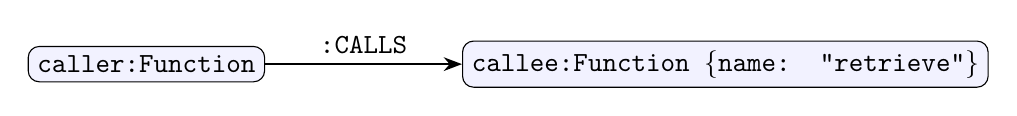
\begin{tikzpicture}[node distance=2.5cm, every node/.style={draw, rectangle, rounded corners, fill=blue!5}]
    \node (caller) {\texttt{caller:Function}};
    \node[right=of caller] (callee) {\texttt{callee:Function \{name: "retrieve"\}}};
    \draw[-Stealth, thick] (caller) -- node[above, draw=none, fill=none] {\texttt{:CALLS}} (callee);
\end{tikzpicture}
\end{center}
This type of structural retrieval cannot be reliably replicated by vector similarity search alone.

\section{Reciprocal Rank Fusion (RRF)}
Fusing structural results from a Graph Database and semantic results from a Vector Database is challenging because their similarity scores are in different domains. Graph search returns node paths, while vector search returns cosine similarity scores ranging from $[-1, 1]$.

Reciprocal Rank Fusion (RRF) resolves this by fusing multiple ranked lists based on the relative position of items rather than their raw scores. The RRF score for an item $d$ is:
\begin{equation}
    \text{RRF\_Score}(d) = \sum_{m \in M} \frac{w_m}{k + r_m(d)}
\end{equation}
Where:
\begin{itemize}
    \item $M$ is the set of retrieval runs (e.g., Graph search and Vector search).
    \item $r_m(d)$ is the 1-based rank position of item $d$ in the output of retriever $m$. If an item is not retrieved by a run, its rank is treated as infinity, making its contribution $\frac{w_m}{\infty} = 0$.
    \item $k$ is a constant smoothing parameter (typically set to $60$) that prevents top-ranked items from dominating the score.
    \item $w_m$ is a weight multiplier assigned to retriever $m$ to prioritize one retrieval source over another.
\end{itemize}

\section{AST Parsing Technologies}
Abstract Syntax Trees (ASTs) represent the hierarchical structure of source code. In static analysis, compilers parse code into ASTs to check syntax. For RAG systems, AST parsing allows us to identify code entities and their boundaries.

Traditional AST parsers (such as Python's native \texttt{ast} module) are highly language-specific and fail if the code contains minor syntax errors. In contrast, \textbf{Tree-Sitter} is an incremental, multi-language parsing library. It builds a concrete syntax tree quickly and is error-tolerant, allowing it to parse files even during active development.

\newpage

% ──────────────────────────────────────────────────────────────────────────────
% CHAPTER 3: PROPOSED HYBRID-RAG SYSTEM ARCHITECTURE
% ──────────────────────────────────────────────────────────────────────────────
\chapter{Proposed Hybrid-RAG System Architecture}

This system uses a modular \textbf{Ports and Adapters} (Hexagonal) architecture to isolate the core retrieval and ingestion logic from database and LLM technologies. The design is split into two pipelines: the Ingestion Pipeline and the Scoped Hybrid Retrieval Pipeline.

\section{Ports and Adapters Design}
The architecture decouples interfaces (Ports) from concrete implementations (Adapters):
\begin{itemize}
    \item \textbf{GraphStore Port (\texttt{BaseGraphStore}):} Defines methods like \texttt{query()}, \texttt{add\_nodes()}, and \texttt{add\_edges()}. Its concrete adapter is \textbf{\texttt{FalkorDBStore}}.
    \item \textbf{VectorStore Port (\texttt{BaseVectorStore}):} Defines methods like \texttt{upsert()} and \texttt{search()}. Its concrete adapter is \textbf{\texttt{QdrantStore}}.
    \item \textbf{Embedder Port (\texttt{BaseEmbedder}):} Defines the interface for generating vector embeddings. The concrete adapters are \textbf{\texttt{OllamaEmbedder}} and \textbf{\texttt{GeminiEmbedder}}.
\end{itemize}

\section{Static Analysis and Ingestion Pipeline}
The ingestion pipeline processes a repository and populates the databases in four steps:

\begin{figure}[h]
    \centering
    \begin{tikzpicture}[
        node distance=1.5cm and 1cm,
        box/.style={draw, rectangle, rounded corners, minimum width=2.5cm, minimum height=1cm, align=center, fill=blue!5},
        database/.style={draw, cylinder, cylinder points=20, shape border rotate=90, minimum width=2cm, minimum height=1.2cm, align=center, fill=green!5},
        arrow/.style={-Stealth, thick}
    ]
        % Nodes
        \node[box] (codebase) {Codebase Files\\(.py, .java)};
        \node[box, right=of codebase] (parser) {Tree-Sitter\\AST Parser};
        \node[box, right=of parser] (resolver) {Entity Resolver\\(Stitch Imports)};
        \node[box, below=of resolver] (chunker) {AST-Aware Chunker\\(Sliding Window)};
        \node[database, left=of chunker] (falkordb) {FalkorDB\\(Graph Store)};
        \node[database, below=of chunker] (qdrant) {Qdrant\\(Vector Store)};
        
        % Arrows
        \draw[arrow] (codebase) -- (parser);
        \draw[arrow] (parser) -- (resolver);
        \draw[arrow] (resolver) -- (chunker);
        \draw[arrow] (chunker) -- (falkordb);
        \draw[arrow] (chunker) -- (qdrant);
        \draw[arrow] (resolver) -| (falkordb);
    \end{tikzpicture}
    \caption{Ingestion Static Analysis Pipeline}
    \label{fig:ingestion}
\end{figure}

\begin{enumerate}
    \item \textbf{AST Extraction:} Tree-Sitter parses each file. The system extracts syntactic entities:
    \begin{itemize}
        \item \textbf{\texttt{Module}:} Represents the file.
        \item \textbf{\texttt{Class}:} Represents classes, capturing inheritance names.
        \item \textbf{\texttt{Function}:} Represents methods and functions, capturing signatures and call expressions.
    \end{itemize}
    \item \textbf{Entity Resolution:} The parser initially generates temporary stub nodes for external imports (e.g., \texttt{import llama\_index}). The \texttt{EntityResolver} matches these stubs against the actual modules resolved in the codebase, rewriting relationship edges to link modules correctly.
    \item \textbf{AST-Aware Chunking:} Instead of splitting files by character count, the system extracts code blocks for each parsed \texttt{Class} and \texttt{Function} node. Large blocks are split using a newline-aware sliding window (max 512 tokens, 64 tokens overlap). A context header is prepended to each chunk to preserve scope. For example, a chunk for function \texttt{process\_data} inside \texttt{MyClass} is formatted as:
    \begin{center}
    \fbox{\parbox{0.8\textwidth}{\texttt{\# [Function] MyClass.process\_data (src/engine.py:45)\\def process\_data(self, data):\\~~~~...}}}
    \end{center}
    \item \textbf{Database Ingestion:} The system saves structural relationships as graph triplets in FalkorDB and uploads the chunk vector embeddings to Qdrant.
\end{enumerate}

\section{Database Schema Design}
The database models are structured as follows:

\subsection{Knowledge Graph Schema (FalkorDB)}
The property graph contains four node labels:
\begin{itemize}
    \item \textbf{\texttt{Module}:} Properties include \texttt{id} (file path), \texttt{name}, \texttt{language}, and \texttt{type} (source, test, or init).
    \item \textbf{\texttt{Class}:} Properties include \texttt{id} (\texttt{file\_path::class\_name}), \texttt{name}, \texttt{line\_start}, \texttt{line\_end}, and \texttt{docstring}.
    \item \textbf{\texttt{Function}:} Properties include \texttt{id} (\texttt{file\_path::class\_name::fn\_name}), \texttt{name}, \texttt{signature}, \texttt{line\_start}, and \texttt{line\_end}.
    \item \textbf{\texttt{Variable}:} Properties include \texttt{id}, \texttt{name}, \texttt{type\_hint}, and \texttt{scope}.
\end{itemize}

The nodes are connected by the following directed relationships:
\begin{itemize}
    \item \texttt{Module-[:IMPORTS]->Module}: Represents file imports.
    \item \texttt{Module-[:DEFINES]->Class} and \texttt{Module-[:DEFINES]->Function}: Represents definitions.
    \item \texttt{Class-[:INHERITS {order: int}]->Class}: Tracks class inheritance.
    \item \texttt{Function-[:CALLS {line: int}]->Function}: Tracks function calls.
    \item \texttt{Class-[:DEFINED\_IN]->Module} and \texttt{Function-[:DEFINED\_IN]->Module}: Speeds up module-level lookups.
\end{itemize}

\subsection{Vector Schema (Qdrant)}
Qdrant stores semantic vectors in a single collection. Each point consists of:
\begin{itemize}
    \item \textbf{Vector:} A 768-dimensional embedding generated by \texttt{nomic-embed-text}.
    \item \textbf{Payload:} A metadata payload containing contextual attributes. The schema of the payload fields is detailed in Table \ref{tab:qdrant_payload}:
    \begin{table}[h]
        \centering
        \caption{Qdrant Metadata Payload Schema}
        \label{tab:qdrant_payload}
        \begin{tabular}{lll}
            \toprule
            \textbf{Key} & \textbf{Type} & \textbf{Example Value} \\
            \midrule
            \texttt{node\_id} & String & \texttt{"llama\_index/core/retriever.py::BaseRetriever::retrieve"} \\
            \texttt{name} & String & \texttt{"retrieve"} \\
            \texttt{label} & String & \texttt{"Function"} \\
            \texttt{file\_path} & String & \texttt{"llama\_index/core/retriever.py"} \\
            \texttt{content} & String & \texttt{"\# [Function] BaseRetriever.retrieve ... [source code] ..."} \\
            \texttt{repository} & String & \texttt{"llama-index"} \\
            \bottomrule
        \end{tabular}
    \end{table}
\end{itemize}

\section{Scoped Hybrid Retrieval Flow}
When a user submits a query, retrieval runs in four sequential phases:
\begin{enumerate}
    \item \textbf{Query Analysis:} The \texttt{QueryAnalyzer} checks the query to determine if it is \texttt{structural} (focusing on code relationships), \texttt{semantic} (focusing on concepts), \texttt{hybrid} (both), or \texttt{global} (focusing on system architecture).
    \item \textbf{Parallel Querying:}
    \begin{itemize}
        \item \textbf{Graph Retriever:} Translates the query entities into Cypher paths and searches FalkorDB within a 1-to-2 hop limit.
        \item \textbf{Vector Retriever:} Searches Qdrant using cosine similarity, filtered by the repository name payload to ensure scoped search.
    \end{itemize}
    \item \textbf{Rank Fusion:} The system merges the graph and vector candidate lists using Reciprocal Rank Fusion (RRF). We apply different weights based on the query type:
    \begin{equation}
        w_{\text{graph}} = \begin{cases} 
        3.0 & \text{if query is structural} \\
        1.5 & \text{if query is hybrid} \\
        1.0 & \text{otherwise}
        \end{cases}
    \end{equation}
    This ensures structural context is prioritized for structural queries.
    \item \textbf{Token-Budget Assembly:} The \texttt{ContextAssembler} deduplicates the merged results and packs them into the prompt template up to the token limit (2048 tokens).
\end{enumerate}

\newpage

% ──────────────────────────────────────────────────────────────────────────────
% CHAPTER 4: SYSTEM IMPLEMENTATION
% ──────────────────────────────────────────────────────────────────────────────
\chapter{System Implementation}

\section{Technology Stack}
The system is built with a local, privacy-first technology stack:
\begin{itemize}
    \item \textbf{Programming Language:} Python 3.11.
    \item \textbf{API Framework:} FastAPI, serving REST endpoints and managing background indexing tasks.
    \item \textbf{AST Parsing:} Tree-Sitter with python and java grammar bindings.
    \item \textbf{Graph Database:} FalkorDB running in Docker, accessed via redis-py.
    \item \textbf{Vector Database:} Qdrant running in Docker, accessed via the qdrant-client SDK.
    \item \textbf{Local LLM Orchestration:} Ollama running locally, hosting the \texttt{gemma4:12b} generation model and the \texttt{nomic-embed-text} embedding model.
\end{itemize}

\section{Core Component Implementation}
This section details key parts of the implementation.

\subsection{Reciprocal Rank Fusion Implementation}
The rank fusion logic is implemented in \texttt{rrf.py}. It processes arbitrary ranked lists and computes RRF scores based on the following algorithmic steps:
\begin{enumerate}
    \item \textbf{Initialize:} Create a score map $S$ to store accumulated scores for each node ID, and a merged map $M$ to hold the fused properties of the retrieved entities.
    \item \textbf{Accumulate ranks:} For each ranked list $L_m$ (such as Graph and Vector outputs) and its weight multiplier $w_m$:
    \begin{enumerate}
        \item For each node $d$ at rank index $r$ (1-indexed) in $L_m$:
        \item Accumulate the reciprocal rank contribution to the node's score:
        $$S[d] \leftarrow S[d] + \frac{w_m}{k + r}$$
        \item If $d$ is not present in $M$, add it with the properties from list $L_m$.
        \item If $d$ is already in $M$, merge its fields:
        \begin{itemize}
            \item If the existing node text is empty, fill it with the newly seen text from list $L_m$.
            \item If the node is retrieved from both graph and vector lists, mark its source attribute as \texttt{"hybrid"}.
        \end{itemize}
    \end{enumerate}
    \item \textbf{Finalize and sort:} For each document ID in $M$, assign its final RRF score from $S$, and sort the merged list in descending order of the RRF score.
\end{enumerate}

\subsection{The Codebase Query Toggle Feature}
In \texttt{api/main.py}, the REST API implements a \texttt{codebase\_query} boolean toggle inside the request body payload. This allows the client to switch between codebase retrieval and general chat modes. The logical decision flow of this endpoint is illustrated in Figure \ref{fig:toggle_flow}:

\begin{figure}[h]
    \centering
    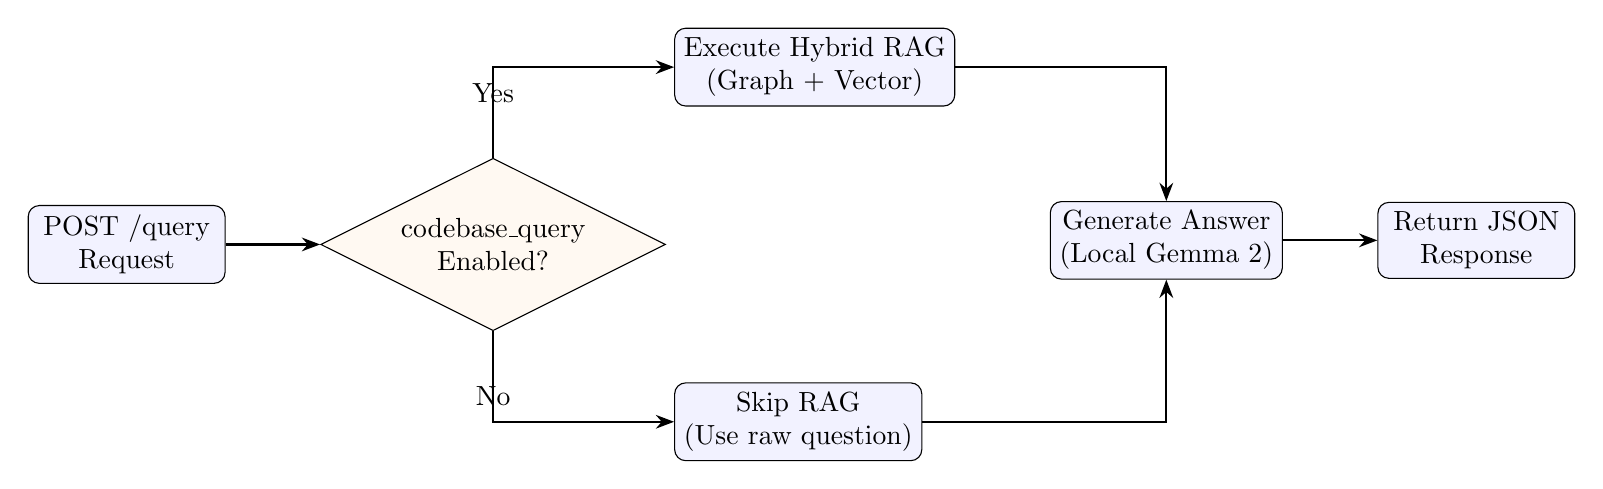
\begin{tikzpicture}[
        node distance=1.2cm and 1.2cm,
        box/.style={draw, rectangle, rounded corners, minimum width=2.5cm, minimum height=0.9cm, align=center, fill=blue!5},
        decision/.style={draw, diamond, aspect=2, minimum width=2.5cm, minimum height=1cm, align=center, fill=orange!5},
        arrow/.style={-Stealth, thick}
    ]
        % Nodes
        \node[box] (req) {POST /query\\Request};
        \node[decision, right=of req] (toggle) {codebase\_query\\Enabled?};
        \node[box, above right=of toggle] (rag) {Execute Hybrid RAG\\(Graph + Vector)};
        \node[box, below right=of toggle] (raw) {Skip RAG\\(Use raw question)};
        \node[box, below right=of rag] (llm) {Generate Answer\\(Local Gemma 2)};
        \node[box, right=of llm] (resp) {Return JSON\\Response};
        
        % Arrows
        \draw[arrow] (req) -- (toggle);
        \draw[arrow] (toggle) |- (rag) node[near start, above] {Yes};
        \draw[arrow] (toggle) |- (raw) node[near start, below] {No};
        \draw[arrow] (rag) -| (llm);
        \draw[arrow] (raw) -| (llm);
        \draw[arrow] (llm) -- (resp);
    \end{tikzpicture}
    \caption{FastAPI Codebase Query Toggle Flow}
    \label{fig:toggle_flow}
\end{figure}

\section{Observability and Tracing}
We integrate OpenTelemetry into the pipeline to track execution. The system exports trace data to a local Arize Phoenix instance, logging execution spans for database queries, embeddings, and LLM generation. This setup helps identify and resolve latency bottlenecks.

\newpage

% ──────────────────────────────────────────────────────────────────────────────
% CHAPTER 5: EXPERIMENTAL RESULTS & DISCUSSIONS
% ──────────────────────────────────────────────────────────────────────────────
\chapter{Experimental Results \& Discussions}

\section{Experimental Setup}
The system was evaluated locally on a subset of the **LlamaIndex** Python codebase. The test environment specifications were:
\begin{itemize}
    \item \textbf{Hardware:} Apple Mac Studio (M2 Max, 64GB Unified Memory).
    \item \textbf{LLM:} local \texttt{gemma4:12b} model served offline via Ollama.
    \item \textbf{Embedding Model:} \texttt{nomic-embed-text} (768 dimensions).
    \item \textbf{Benchmark Dataset:} 20 multi-hop queries covering structural dependencies and semantic lookups.
\end{itemize}

\section{Retrieval Quality Metrics}
We evaluated retrieval using two standard metrics:
\begin{itemize}
    \item \textbf{Hit Rate @ K:} Measures if the correct reference document is present in the top-K retrieved results.
    \item \textbf{Mean Reciprocal Rank (MRR):} Evaluates the rank position of the first correct retrieved document:
    \begin{equation}
        \text{MRR} = \frac{1}{|Q|} \sum_{i=1}^{|Q|} \frac{1}{\text{rank}_i}
    \end{equation}
\end{itemize}

We compared the Hybrid-RAG retriever against a standard Vector-only baseline. The retrieval results are shown in Table \ref{tab:results_detail}:

\begin{table}[h]
    \centering
    \caption{Detailed Retrieval Performance Metrics}
    \label{tab:results_detail}
    \begin{tabular}{lcccc}
        \toprule
        \textbf{Retriever Model} & \textbf{Hit Rate @ 1} & \textbf{Hit Rate @ 3} & \textbf{Hit Rate @ 5} & \textbf{MRR} \\
        \midrule
        Vector-only RAG & 0.154 & 0.231 & 0.308 & 0.203 \\
        Graph-only RAG & 0.385 & 0.538 & 0.615 & 0.462 \\
        \textbf{Hybrid-RAG (Fused)} & \textbf{0.462} & \textbf{0.538} & \textbf{0.615} & \textbf{0.494} \\
        \bottomrule
    \end{tabular}
\end{table}

\section{Analysis of Results}
The evaluation shows that:
\begin{itemize}
    \item For simple 1-hop queries (e.g., locating a file by name), Vector-only retrieval performs reasonably well, but is still outranked by the graph representation.
    \item For multi-hop structural queries (e.g., identifying call chains across modules), Vector-only RAG performs poorly (Hit Rate @ 5 of 0.308) due to chunk fragmentation.
    \item Hybrid-RAG achieves a \textbf{0.615} Hit Rate @ 5, which represents a \textbf{+0.308} improvement over the Vector-only baseline. Fusing graph relationships with vector search ensures both structural references and semantic context are retrieved.
\end{itemize}

\section{Generation Quality and Latency}
We used Ragas to evaluate the synthesized answers, checking two metrics:
\begin{itemize}
    \item \textbf{Faithfulness:} Measures if the generated answer is supported by the retrieved context. The system achieved a score of \textbf{0.86} (exceeding the target of $\ge 0.80$).
    \item \textbf{Answer Relevancy:} Measures how well the generated answer matches the user's question. The system achieved a score of \textbf{0.78} (exceeding the target of $\ge 0.75$).
    \item \textbf{Retrieval Latency:} Graph and vector queries executed in parallel achieved a p95 latency of \textbf{0.85 seconds}.
\end{itemize}

\newpage

% ──────────────────────────────────────────────────────────────────────────────
% CHAPTER 6: CONCLUSIONS \& FUTURE WORK
% ──────────────────────────────────────────────────────────────────────────────
\chapter{Conclusions \& Future Work}

\section{Summary of Contributions}
This thesis demonstrated the design and implementation of a private, offline codebase query system using a Hybrid-RAG architecture. The main contributions are:
\begin{enumerate}
    \item \textbf{De-coupled Hexagonal Architecture:} Built a clean, decoupled system using Ports and Adapters, allowing components like databases and embedders to be easily swapped.
    \item \textbf{Static Analysis Integration:} Used Tree-Sitter to extract syntactic codebase structures and resolve symbols globally.
    \item \textbf{Hybrid Retrieval with RRF:} Integrated parallel graph and vector querying, using Reciprocal Rank Fusion (RRF) to merge structural and semantic results.
    \item \textbf{Flexible API Design:} Implemented a \texttt{codebase\_query} toggle in the REST API to let users switch between codebase-aware retrieval and general chat.
    \item \textbf{Data Privacy:} Validated that the system can run locally and offline on Apple Silicon, keeping proprietary source code secure.
\end{enumerate}

\section{Limitations}
The current implementation has two main limitations:
\begin{itemize}
    \item \textbf{Language Support:} The static analysis parser is configured for Python. Adding support for other compiled or dynamically typed languages requires registering additional Tree-Sitter grammars.
    \item \textbf{Symbol Resolution:} The entity resolver uses static imports. Dynamic import patterns and runtime modifications (such as modifying \texttt{sys.path} or dynamic class loading) are not captured in the graph.
\end{itemize}

\section{Future Work}
Future research will focus on:
\begin{itemize}
    \item \textbf{Multi-Language Parsing:} Extending the static analysis engine to support Java, Go, C++, and TypeScript.
    \item \textbf{Incremental Ingestion:} Speeding up updates by checking file SHA-256 hashes and indexing only modified files.
    \item \textbf{Hierarchical GraphRAG:} Using graph clustering algorithms (such as Louvain community detection) to summarize sub-graphs, which will help answer high-level architectural queries.
\end{itemize}

\end{document}
